

\input{../Latex_Templates/Preamble_Presentation}


%%%%% TITLE PAGE

% \subject{}
\title{Stagnation points of harmonic vector fields and the domain topology}
\subtitle{Some applications of Morse theory}
%\subtitle{Blatt 0}
\author{Theo Koppenhöfer}
\date{\today}

\addbibresource{bibliography.bib}
\graphicspath{{../Plots/}}
\graphicspath{{../Figures/}}


\begin{document}

% \frame[plain]

% Frame 2
\frame[plain]{\titlepage}

% Frame 3
% \frame[plain]{\tableofcontents }

\section{Introduction}


\section{Flowthrough with stagnation point}

\begin{frame}
  \begin{question}[Flowthrough with stagnation point] \label{qu:flowthroughStagnationPoint}
		Does there exist a domain $X\subset\R^d$ homeomorphic to a ball and a harmonic vector field $u\colon X\to\R^d$ on $X$ such that
		\begin{enumerate}
		  \item $u$ has an interior stagnation point
		  \item the boundaries on which $u$ enters and leaves the region are simply connected?
		\end{enumerate}
	\end{question}
\end{frame}

\begin{frame}
	\begin{question}[Flowthrough with stagnation point] \label{qu:flowthroughStagnationPoint}
		Does there exist a domain $X\subset\R^d$ homeomorphic to a ball and a harmonic vector field $u\colon X\to\R^d$ on $X$ such that
		\begin{enumerate}
		  \item $u$ has an interior stagnation point
		  \item the boundaries on which $u$ enters and leaves the region are simply connected?
		\end{enumerate}
	\end{question}
  \begin{answer}
  \begin{itemize}
    \item $d=2$ dimensions: Not possible (known).
    \item cylinders in $d=3$ dimensions: Not possible (known).
    \item $d=3$ dimensions: Number of stagnation points has to be even.
    \item $d=4$ dimensions: Possible for $X=B_1$, $u=\nabla f$ with $$f=x_1^2+x_2^2-x_3^2-x_4^2\,.$$
  \end{itemize}
\end{answer}
\end{frame}

\begin{frame}
  \begin{figure}
    \centering
    \input{../Figures/n3_cylinder.pdf_tex}
    \caption{This kind of situation is not possible.}
    \label{fi:n3_cylinder}
  \end{figure}
\end{frame}

\begin{frame}
  But if one allows for holes in $d=2$ dimensions it becomes possible.
  \begin{figure}
    \centering
    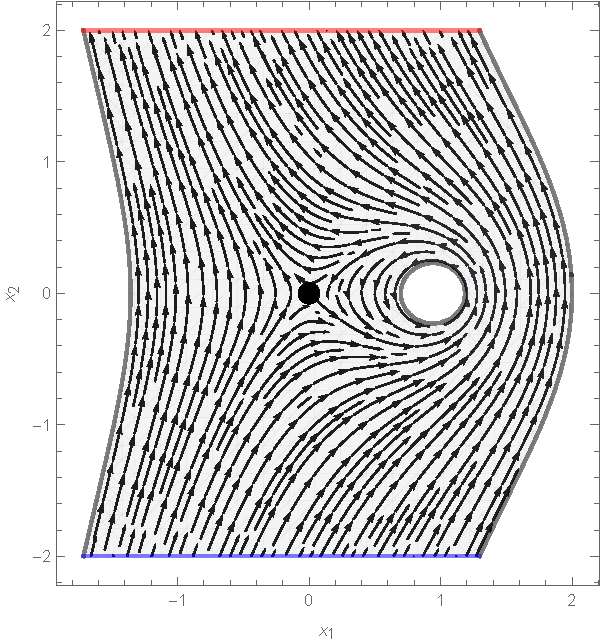
\includegraphics[width=0.5\textwidth]{../Plots/n2_hvf_InflowOutflow_asymmetric_gray_2.pdf}
    % 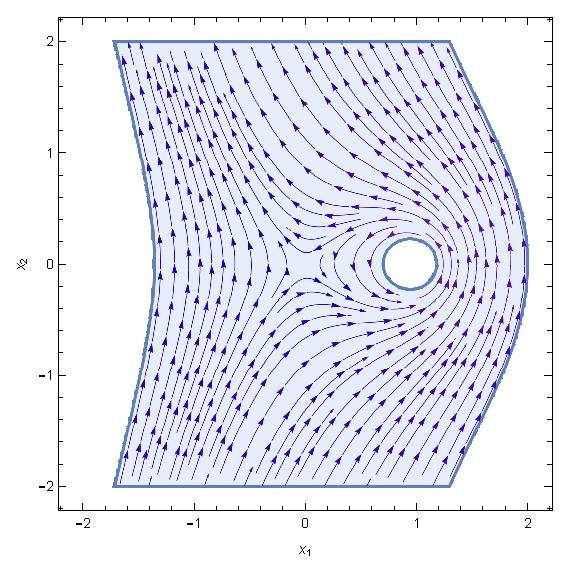
\includegraphics[width=0.6\textwidth]{../Plots/HarmonicVectorFields_gr3.eps}
    \caption{A plot of $u=\nabla^\perp\psi$ in the region $\psi^{-1}\brk*{[-0.5,2]}\cap \brk*{\R\times[-2,2]}$.
    Here $\psi\leftdef\Phi_2\brk*{x-e_1}+x_1$.}
    \label{pl:n2_hvf_InflowOutflow_asymmetric_single}
  \end{figure}
\end{frame}

\begin{frame}
  For $d=3$ dimensions we have for $r$ sufficiently large the example $X=B_r$, $u=\nabla f$ with
  \begin{align*}
    f=\frac{x_1^2}{2}-\frac{x_1^3}{3}-\frac{x_1x_2^2}{2}+x_1x_2^2+x_2x_3
  \end{align*}
\end{frame}

\begin{frame}
  \begin{figure}
    \centering
    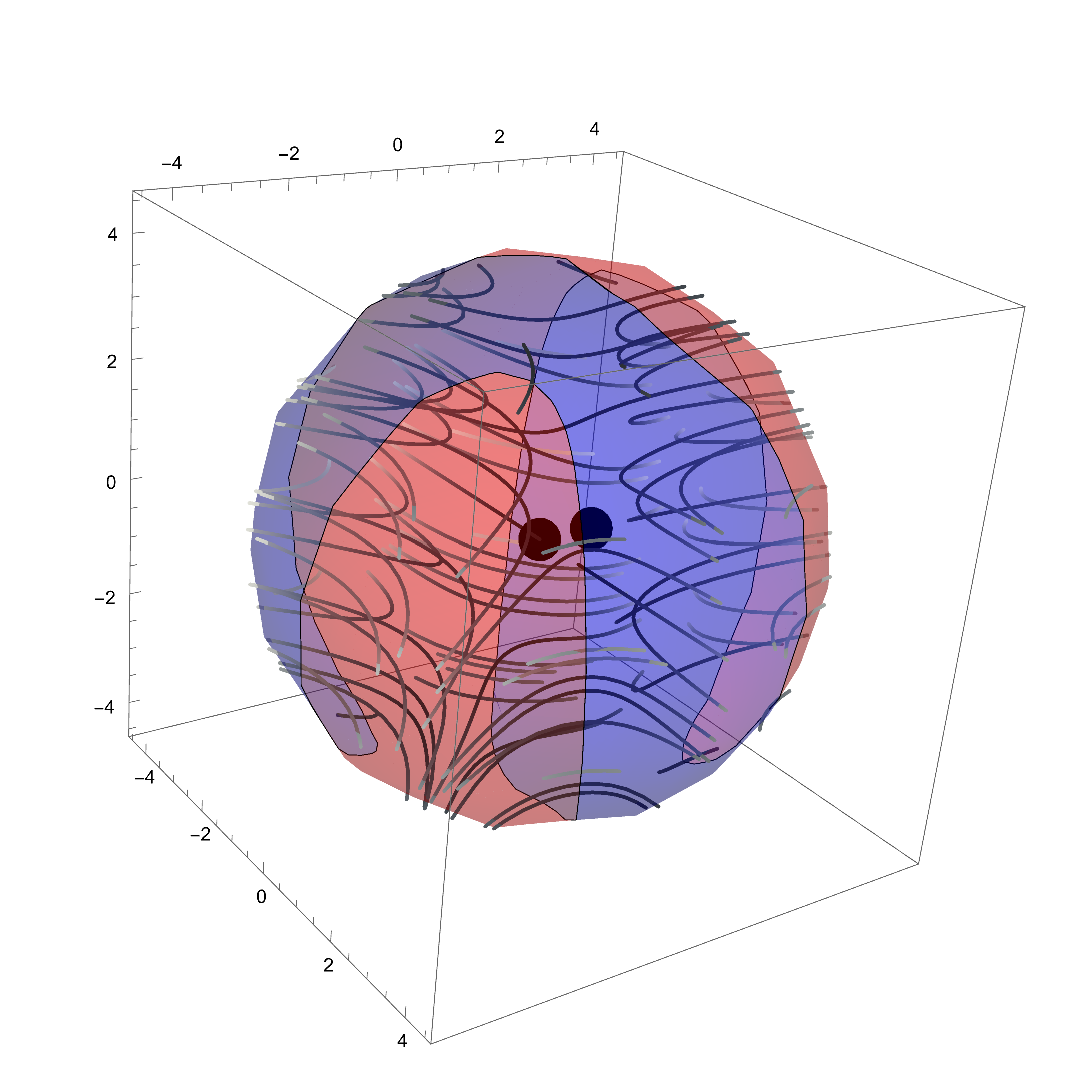
\includegraphics[width=0.6\textwidth]{../plots/n3_hf_inflowOutflow_Ball_overview.pdf}
    \caption{A stream plot of the function $u$. The interior stagnation points are highlighted in black.
    $\Sigma^+$ is shaded red, $\Sigma^-$ blue.}
    \label{pl:n3_hf_inflowOutflowStagnationPoint_overview}
  \end{figure}
\end{frame}

\begin{frame}
  \begin{figure}
    \centering
    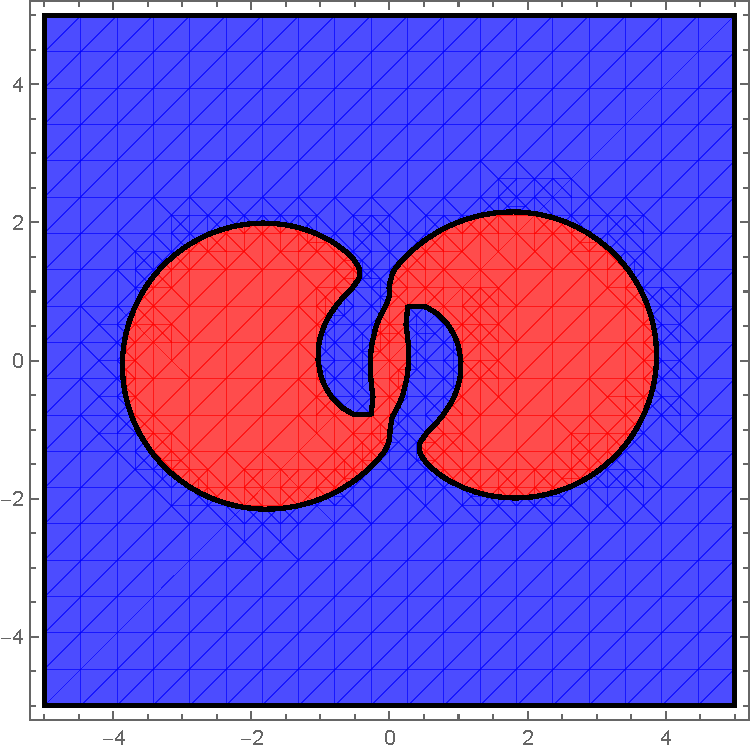
\includegraphics[width=0.6\textwidth]{../plots/n3_hf_inflowOutflow_Ball_Surface_2.pdf}
    \caption{Stereographic projection of the surface $\Sigma$. $\Sigma^+$ is shaded red, $\Sigma^-$ blue.}
    \label{pl:n3_hf_inflowOutflowStagnationPoint_Surface}
  \end{figure}
\end{frame}

\begin{frame}
  One can perturb this solution to show that there exists a harmonic vector field
  on $B_r$ with interior stagnation point such that $\Sigma^+$ and $\Sigma^-$ have positive distance
  from one another and are simply connected.
\end{frame}

\section{Harmonic vector fields without inflow or outflow}

\begin{frame}
  \begin{question}[Harmonic vector fields without inflow or outflow]
    Let $u$ be a harmonic vector field in a domain $X$ such that at every boundary point it is tangential to the boundary
    and non-vanishing.
    What can be said about the relation between the number of stagnation points and the domain topology?
  \end{question}
\end{frame}

\begin{frame}
  In $d=2$ dimensions one essentially has the relation
  \begin{align*}
    M=\chi\brk*{X}
  \end{align*}
  where $M$ is the number of stagnation points and $\chi\brk*{X}$ the Euler characteristic of $X$.
\end{frame}

\begin{frame}
  \begin{figure}
    \centering
    % 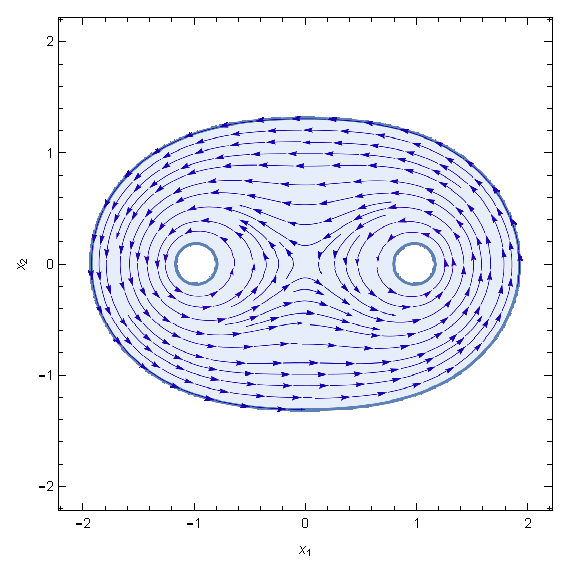
\includegraphics[width=0.6\textwidth]{../Plots/HarmonicVectorFields_gr1.eps}
    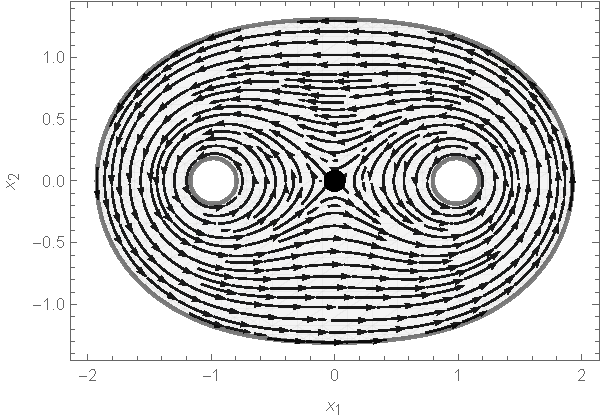
\includegraphics[width=0.6\textwidth]{../Plots/n2_hvf_noInflowNoOutflow_symmetric_gray_2.pdf}
    \caption{A plot of $u=\nabla^\perp\psi$ in the domain $\psi^{-1}\brk*{[-1,1]}$.
      Here $\psi\leftdef\Phi_2\brk*{x-e_1}+\Phi_2\brk*{x+e_1}$.}
    \label{pl:n2_hvf_noInflowNoOutflow}
  \end{figure}
\end{frame}

\begin{frame}
  In $d=3$ dimensions one has essentially an even number of stagnation points.
\end{frame}

\section{Sources}

\begin{frame}[allowframebreaks]
	\frametitle{Sources}
	\nocite{*}

	% \bibliographystyle{plain}
	\setbeamertemplate{bibliography item}[text]
	% \bibliography{bibliographyFile}
	\printbibliography
\end{frame}

\begin{frame}[plain]
	\begin{center}
		\Large{{Thank you for your attention.}}
	\end{center}
\end{frame}

% \frame[plain]

\end{document}